\documentclass{beamer}
\usepackage{amsmath}
\usepackage{graphicx}
\usepackage{animate}
\usepackage{tikz}
\usetikzlibrary{decorations.pathmorphing}
\usetheme{Berlin}
\usepackage{pgfplots}
\pgfplotsset{compat=1.18}
\usepackage{multimedia}

\usetikzlibrary{shapes.geometric, arrows.meta, positioning}





\title{Die Schrödinger-Gleichung: Herleitung und Anwendung}
\author{Lucien \& Jan}
\date{\today}

\begin{document}

    \begin{frame}
        \titlepage
    \end{frame}

%    \begin{frame}{Wellenpaket-Animation (1D-Zeitentwicklung)}
    \centering
    \begin{animateinline}[
        controls={play, step, stop},
        loop,
        poster=first,
        width=0.8\textwidth
    ]{10} % 10 Frames pro Sekunde
        \multiframe{20}{rt=0.0+0.25} % 20 Frames von t=0 bis t=5
        {
            \begin{tikzpicture}
                \begin{axis}[
                    width=0.8\textwidth,
                    height=6cm,
                    xlabel=$x$,
%                        ylabel=$|\psi(x,t)|^2$,
                    ylabel=$|\psi (x\,t)|^2$,
                    xmin=-3, xmax=3,
                    ymin=0, ymax=1.2,
                    grid=major
                ]
                    % Hüllkurve
                    \addplot[red!50, thick, domain=-3:3, samples=50] {
                        exp(-(x - 0.5*\rt)^2)
                    };

                    % Wellenpaket mit Oszillationen
                    \addplot[blue, thick, domain=-3:3, samples=100] {
                        exp(-(x - 0.5*\rt)^2) * (1 + 0.3*cos(deg(5*x - 2*\rt)))
                    };

%                         Zeitmarker
                    \node[draw] at (axis cs:2,1) {$t = \pgfmathprintnumber{\rt}$};
                \end{axis}
            \end{tikzpicture}
        }
    \end{animateinline}

%        \begin{itemize}
%            \item Klicken Sie auf "Play" um die Zeitentwicklung zu starten
%            \item Geschwindigkeit mit "+/-" anpassbar
%            \item Deutlich sichtbar: Bewegung + Dispersion + Interferenz
%        \end{itemize}
\end{frame}

\begin{frame}{Wellenpaket-Animation (2D-Zeitentwicklung)}
    \centering
    \begin{animateinline}[
        controls={play, step, stop},
        loop,
        poster=first,
        width=0.8\textwidth
    ]{10} % 10 Frames pro Sekunde
        \multiframe{20}{rt=0.0+0.25} % 20 Frames von t=0 bis t=5
        {
            \centering
            \begin{tikzpicture}
                \begin{axis}
                    [
                    width=0.8\textwidth,
                    height=6cm,
                    colormap/viridis,
                    view = {45}{30},
                    xlabel = $x$,
                    ylabel = $y$,
                    axis line style={draw=none},
                    zlabel = {Wahrscheinlichkeitsdichte $|\psi(x,y)|^2$},
                    label style = {sloped},
                    grid = major,
                    grid style = {dashed, gray!30},
                    tick label style = {font=\scriptsize},
                    title = {Moduliertes Gaußsches Wellenpaket},
                    title style = {font=\small},
                    colorbar,
                    colorbar style={
                        title=Intensität,
                        yticklabel style={/pgf/number format/.cd,fixed,precision=2}
                    }
                    ]

                    % Hüllkurve
                    \addplot3[
                    surf,
                    shader = interp,
                    samples = 20,
                    domain = -3:3,
                    y domain = -3:3,
%                point meta=abs,
                    ] {
%                    exp(-(x^2 + y^2))       % Gaußscher Kern
%                    * (1 + 0.4*cos(6*x))    % Wellenmodulation
%                    * (1 + 0.4*cos(6*y))    % 2D-Interferenzmuster
%                    exp(-(x^2 + y^2))* (1 + 0.4*cos(6*x))* (1 + 0.4*cos(6*y))
%                        (1 + 0.4*cos(6* deg(x)))* (1 + 0.4*cos(6*deg(y))) * exp(-(x^2 + y^2))
                        exp(-((x - 0.5*\rt)^2 + (y)^2))
                    };


%                    (1 + 0.4*cos(6* deg(x)))* (1 + 0.4*cos(6*deg(y))) * exp(-(x^2 + y^2))
%                    % Hüllkurve
%                    \addplot[red!50, thick, domain=-3:3, samples=50] {
%                        exp(-(x - 0.5*\rt)^2)
%                    };

%                    % Wellenpaket mit Oszillationen
%                    \addplot[blue, thick, domain=-3:3, samples=100] {
%                        exp(-((x - 0.5*\rt)^2)) * (1 + 0.3*cos(deg(5*x - 2*\rt)))
%                    };

%                    \node[white,font=\tiny] at (axis cs:-2.5,-2.5,0.7)
%                        {$\psi(x,y) = e^{-(x^2+y^2)}(1 + 0.4\cos 6x)(1 + 0.4\cos 6y)$};
                \end{axis}
%            \end{tikzpicture}
%            \begin{tikzpicture}
%                \begin{axis}[
%                    width=0.8\textwidth,
%                    height=6cm,
%                    xlabel=$x$,
%%                        ylabel=$|\psi(x,t)|^2$,
%                    ylabel=$|\psi (x\,t)|^2$,
%                    xmin=-3, xmax=3,
%                    ymin=0, ymax=1.2,
%                    grid=major
%                ]
%
%%                    (1 + 0.4*cos(6* deg(x)))* (1 + 0.4*cos(6*deg(y))) * exp(-(x^2 + y^2))
%                    % Hüllkurve
%                    \addplot[red!50, thick, domain=-3:3, samples=50] {
%                        exp(-(x - 0.5*\rt)^2)
%                    };
%
%                    % Wellenpaket mit Oszillationen
%                    \addplot[blue, thick, domain=-3:3, samples=100] {
%                        exp(-((x - 0.5*\rt)^2)) * (1 + 0.3*cos(deg(5*x - 2*\rt)))
%                    };
%
%%                         Zeitmarker
%                    \node[draw] at (axis cs:2,1) {$t = \pgfmathprintnumber{\rt}$};
%                \end{axis}
            \end{tikzpicture}
        }
    \end{animateinline}

%        \begin{itemize}
%            \item Klicken Sie auf "Play" um die Zeitentwicklung zu starten
%            \item Geschwindigkeit mit "+/-" anpassbar
%            \item Deutlich sichtbar: Bewegung + Dispersion + Interferenz
%        \end{itemize}
\end{frame}

    \begin{frame}{Was ist die Schrödinger-Gleichung?}
        \begin{itemize}
            \item Grundgleichung der Quantenmechanik
            \item Beschreibt, wie sich Quantenzustände mit der Zeit entwickeln
            \item Zeitunabhängige Form: $\hat{H}\psi = E\psi$
        \end{itemize}
    \end{frame}

    \begin{frame}{Die zeitunabhängige Schrödinger-Gleichung}
        \[
            -\frac{\hbar^2}{2m}\frac{d^2\psi}{dx^2} + V(x)\psi(x) = E\psi(x)
        \]
        \begin{itemize}
            \item $\hbar$: Reduziertes Planck'sches Wirkungsquantum
            \item $m$: Teilchenmasse
            \item $V(x)$: Potenzialenergie
            \item $E$: Gesamtenergie des Teilchens
        \end{itemize}
    \end{frame}


    % Folie 1: Energieerhaltung (klassisch vs. quantenmechanisch)
    \begin{frame}{Von der klassischen Physik zur Quantenmechanik}
        \textbf{Klassische Energie (Teilchen):}
        \[
            E = \underbrace{\frac{p^2}{2m}}_{\text{kinetisch}} + \underbrace{V(x)}_{\text{potentiell}}
        \]

        \textbf{Quantenmechanik (Welle):}
        \begin{itemize}
            \item Teilchen verhält sich wie eine Welle (De-Broglie: $p = \hbar k$)
            \item \alert{Problem:} Wie übersetzt man $p^2$ in die "Wellensprache"?
        \end{itemize}
    \end{frame}

    \begin{frame}{Herleitung von $\hat{p}$}
        \textbf{De Broglie: } $k=\hbar k$\\
        \textbf{Wellenfunktion: } $\psi (x)=e^{ikx}=cos(kx)+i sin(kx)$\\\

        \begin{align*}
            \psi '(x)&=ike^{ikx}=ik\psi(x)\\
            \underbrace{-i\hbar\frac{d}{dx}}_{\hat{p}}\psi (x) &=-i \cdot i k\hbar\psi(x)=\underbrace{k\hbar}_{p}\psi(x)\\
            \Rightarrow \hat{p}\psi(x)&=p\psi(x)
        \end{align*}
    \end{frame}

% Folie 1: Einführung des Impulsoperators (Grundlagen)
    \begin{frame}{Der Impulsoperator – Bausteine erklärt}
        \textbf{Alle Symbole im Detail:}
        \[
            \hat{p} = -i\hbar \frac{d}{dx}
        \]
        \begin{itemize}
            \item $\psi(x)$: Wellenfunktion \\
            \footnotesize (Beschreibt den Zustand des Teilchens; $|\psi(x)|^2$ = Aufenthaltswahrscheinlichkeit)

            \item $\hbar$: Reduziertes Planck'sches Wirkungsquantum \\
            \footnotesize (Naturkonstante $\approx 1.055 \times 10^{-34}$ Js; "Quantenwirkungs-Einheit")

            \item $i$: Imaginäre Einheit ($i^2 = -1$) \\
            \footnotesize (Mathematisches Werkzeug für Wellenbeschreibung; ermöglicht Rotation in der komplexen Ebene)

            \item $\frac{d}{dx}$: Ableitung nach dem Ort \\
            \footnotesize (Misst die "Änderungsrate" von $\psi$; hier: Wie stark die Welle an der Stelle $x$ gekrümmt ist)
        \end{itemize}
    \end{frame}

% Folie 2: Warum funktioniert dieser Operator? (Beispiel mit ebener Welle)
    \begin{frame}{Test am Beispiel: Ebene Welle}
        \textbf{Versuch:} Wir nehmen eine einfache Welle $\psi(x) = e^{ikx}$ \\
        \textbf{Ziel:} Zeigen, dass $\hat{p}\psi = p\psi$ (Impuls-Eigenzustand)

        \[
            \hat{p}\psi = -i\hbar \frac{d}{dx} \underbrace{e^{ikx}}_{\text{Wellenform}}
        \]

        \begin{itemize}
            \item $k$: Wellenzahl \\
            \footnotesize (Maß für "Wie viele Wellenberge pro Meter": $k = \frac{2\pi}{\lambda}$)

            \item Ableitung: $\frac{d}{dx}e^{ikx} = ik e^{ikx}$ \\
            \footnotesize (Die Ableitung "zieht" den Faktor $ik$ nach vorne – typisch für Exponentialfunktionen)

            \item Ergebnis: $-i\hbar (ik e^{ikx}) = \hbar k e^{ikx}$ \\
            \footnotesize ($i \cdot i = -1$ hebt das Minus auf; $\hbar k$ ist der Impuls $p$!)
        \end{itemize}

        \textbf{Fazit:} $\hat{p}\psi = (\hbar k)\psi = p\psi$ \quad (De-Broglie: $p = \hbar k$)
    \end{frame}

% Folie 3: Kinetische Energie herleiten
    \begin{frame}{Von Impuls zu kinetischer Energie}
        \textbf{Schritt-für-Schritt:}
        \begin{enumerate}
            \item Klassisch: $K = \frac{p^2}{2m}$
            \item Quantenmechanisch: $p^2$ wird zum Operator $\hat{p}^2$
            \[
                \hat{p}^2\psi = (-i\hbar \frac{d}{dx})(-i\hbar \frac{d}{dx}\psi) = -\hbar^2 \frac{d^2\psi}{dx^2}
            \]
            \item Kinetische Energie-Operator:
            \[
                \hat{K} = \frac{\hat{p}^2}{2m} = -\frac{\hbar^2}{2m}\frac{d^2}{dx^2}
            \]
        \end{enumerate}
        \textbf{Merksatz:} Die 2.
        Ableitung der Wellenfunktion beschreibt die \alert{"Krümmung"} – je stärker gekrümmt, desto höhere kinetische Energie!
    \end{frame}

% Folie 4: Gesamtgleichung zusammenbauen
    \begin{frame}{Zusammenfügen der Energieanteile}
        \textbf{Gesamtenergie $E = K + V$ wird zur Operatorgleichung:}
        \[
            \underbrace{-\frac{\hbar^2}{2m}\frac{d^2\psi}{dx^2}}_{\hat{K}\psi} + \underbrace{V(x)\psi}_{\hat{V}\psi} = \underbrace{E\psi}_{\text{Gesamtenergie}}
        \]

        \textbf{Analog zur klassischen Physik:}
        \begin{itemize}
            \item $V(x)\psi$: "Wo das Teilchen sein darf" (Potenzial wirkt wie eine Landschaft)
            \item $-\frac{\hbar^2}{2m}\psi''$: "Wie wild es vibriert" (Krümmung $\sim$ Bewegungsenergie)
        \end{itemize}
    \end{frame}


    \begin{frame}{Elektronen-Wellenfunktion im Grundzustand}
        \centering
        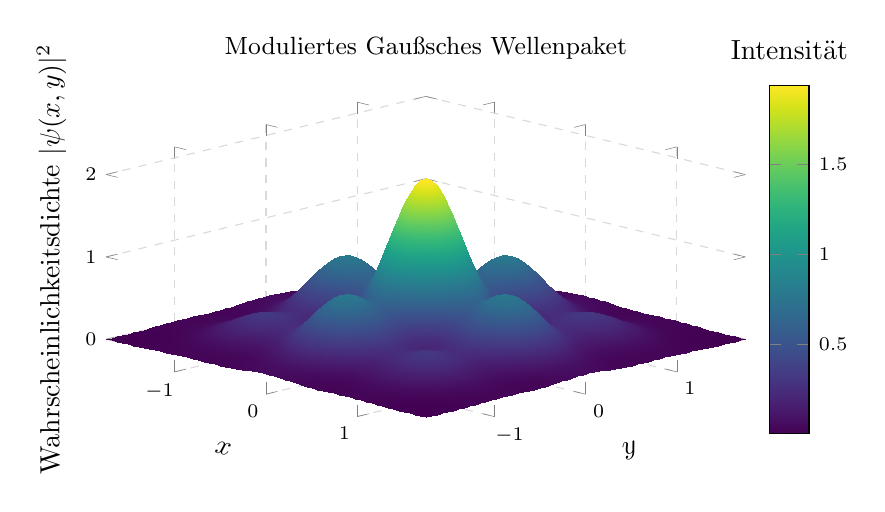
\begin{tikzpicture}
            \begin{axis}
                [
                width=0.8\textwidth,
                height=6cm,
                colormap/viridis,
                view = {45}{30},
                xlabel = $x$,
                ylabel = $y$,
                axis line style={draw=none},
                zlabel = {Wahrscheinlichkeitsdichte $|\psi(x,y)|^2$},
                label style = {sloped},
                grid = major,
                grid style = {dashed, gray!30},
                tick label style = {font=\scriptsize},
                title = {Moduliertes Gaußsches Wellenpaket},
                title style = {font=\small},
                colorbar,
                colorbar style={
                    title=Intensität,
                    yticklabel style={/pgf/number format/.cd,fixed,precision=2}
                }
                ]
                \addplot3[
                surf,
                shader = interp,
                samples = 60,
                domain = -1.75:1.75,
                y domain = -1.75:1.75,
%                point meta=abs,
                ] {
%                    exp(-(x^2 + y^2))       % Gaußscher Kern
%                    * (1 + 0.4*cos(6*x))    % Wellenmodulation
%                    * (1 + 0.4*cos(6*y))    % 2D-Interferenzmuster
%                    exp(-(x^2 + y^2))* (1 + 0.4*cos(6*x))* (1 + 0.4*cos(6*y))
                    (1 + 0.4*cos(6* deg(x)))* (1 + 0.4*cos(6*deg(y))) * exp(-(x^2 + y^2))
                };

                \node[white,font=\tiny] at (axis cs:-2.5,-2.5,0.7)
                    {$\psi(x,y) = e^{-(x^2+y^2)}(1 + 0.4\cos 6x)(1 + 0.4\cos 6y)$};
            \end{axis}
        \end{tikzpicture}
    \end{frame}


% Folie 5: Visualisierung der Terme
%    \begin{frame}{Was bedeuten die Terme?}
%        \centering
%        \includegraphics[width=0.8\textwidth]{potential_well.png}  % Falls ein Bild vorhanden ist
%
%        \textbf{Beispiel Teilchen im Kasten:}
%        \begin{itemize}
%            \item \textcolor{blue}{$V(x)=0$ im Kasten}: Nur kinetische Energie ($\psi$ ist gekrümmt)
%            \item \textcolor{red}{$V(x)=\infty$ außen}: $\psi=0$ (Teilchen kann nicht entkommen)
%        \end{itemize}
%    \end{frame}

    \begin{frame}{Unser Problem}
        \begin{columns}
            \column{0.5\textwidth}
            \begin{itemize}
                \item Elektron bei $x_0$ links der Wand
                \item Potenzialwand von $x_1$ bis $x_2$
                \item $V(x) = \begin{cases}
                                  0 & x < x_1 \\
                                  E_0 & x_1 \leq x \leq x_2 \\
                                  0 & x > x_2
                \end{cases}$
            \end{itemize}

            \column{0.5\textwidth}
            \scalebox{0.7}{
                \begin{tikzpicture}
                    \begin{axis}
                        [
                        axis x line=middle,
                        axis y line=middle,
                        xlabel={$x$},
                        ylabel={$V(x)$},
                        ymin=0, ymax=1.5,
                        xmin=0, xmax=3,
                        xtick={-1,0,1,2,3},
                        ytick={0,1},
                        yticklabels={$0$, $E_0$},
                        domain=-1:3,
                        samples=100
                        ]
                        \addplot[thick, blue] coordinates {(-1,0) (1,0)};
                        \addplot[thick, blue] coordinates {(1,1) (2,1)};
                        \addplot[thick, blue] coordinates {(2,0) (3,0)};
                    \end{axis}
                \end{tikzpicture}
            }
        \end{columns}
    \end{frame}


    \begin{frame}{Lösungsansatz: Bereich I ($x < x_1$)}
        \[
            -\frac{\hbar^2}{2m}\psi'' = E\psi \Rightarrow \psi'' = -k^2\psi
        \]
        Lösung:
        \[
            \psi_I(x) = Ae^{ikx} + Be^{-ikx}
        \]
        \begin{itemize}
            \item $k = \sqrt{2mE}/\hbar$
            \item $Ae^{ikx}$: Einlaufende Welle
            \item $Be^{-ikx}$: Reflektierte Welle
        \end{itemize}
    \end{frame}

    \begin{frame}{Bereich II ($x_1 <= x <= x_2$)}
        \[
            -\frac{\hbar^2}{2m}\psi'' + E_0\psi = E\psi \Rightarrow \psi'' = \kappa^2\psi
        \]
        mit $\kappa = \sqrt{2m(E_0 - E)}/\hbar$

        Lösung:
        \[
            \psi_{II}(x) = Ce^{\kappa x} + De^{-\kappa x}
        \]
        Exponentielle Abnahme/Zunahme der Wellenfunktion!
    \end{frame}

    \begin{frame}{Bereich III ($x > x_2$)}
        \[
            \psi'' = -k^2\psi
        \]
        Lösung:
        \[
            \psi_{III}(x) = Fe^{ikx}
        \]
        \begin{itemize}
            \item Nur durchgehende Welle
            \item Keine Reflexion im Unendlichen
        \end{itemize}
    \end{frame}

    \begin{frame}{Randbedingungen}
        An den Übergängen $x_1$ und $x_2$:
        \begin{enumerate}
            \item Stetigkeit der Wellenfunktion
            \item Stetigkeit der Ableitung
        \end{enumerate}

        Für $x = x_1 = 0$:
        \[
            \begin{cases}
                \psi_I(0) = \psi_{II}(0) \\
                \psi_I'(0) = \psi_{II}'(0)
            \end{cases}
        \]

        Für $x = x_2 = L$:
        \[
            \begin{cases}
                \psi_{II}(L) = \psi_{III}(L) \\
                \psi_{II}'(L) = \psi_{III}'(L)
            \end{cases}
        \]
    \end{frame}

    \begin{frame}{Gleichungssystem lösen (Beispielwerte)}
        Annahme:
        \begin{itemize}
            \item $2m/\hbar^2 = 1$
            \item $E = 1$, $E_0 = 2$ ⇒ $\kappa = 1$
            \item $L = 1$
        \end{itemize}

        Gleichungen werden:
        \[
            \begin{cases}
                A + B = C + D \\
                i(A - B) = C - D \\
                Ce + D/e = Fe^i \\
                Ce - D/e = iFe^i
            \end{cases}
        \]
    \end{frame}

    \begin{frame}{Lösungsschritte}
        \begin{enumerate}
            \item Letzte zwei Gleichungen nach $C$ und $D$ auflösen
            \item In erste Gleichung einsetzen
            \item System für $A$, $B$ und $F$ lösen
            \item Transmission: $T = |F/A|^2$
        \end{enumerate}

%        Ergebnis:
%        \[
%            T \approx 42\% \quad R \approx 58\%
%        \]
    \end{frame}

    \begin{frame}{Exakte Transmissionsformel}
        Allgemeine Lösung für beliebige \( E_0 \) und \( L \):
        \[
            T = \frac{1}{1 + \frac{E_0^2 \sinh^2(\kappa L)}{4E(E_0 - E)}}
        \]
        \begin{itemize}
            \item \( \kappa = \sqrt{\frac{2m(E_0 - E)}{\hbar^2}} \) (Einheit: \( \text{m}^{-1} \))
            \item \( \sinh(x) = \frac{e^x - e^{-x}}{2} \) (hyperbolischer Sinus)
            \item \( E_0 \): Höhe der Potenzialbarriere (Einheit: Joule, J)
            \item \( L \): Breite der Potenzialbarriere (Einheit: Meter, m)
            \item \( m \): Masse des Teilchens (Einheit: Kilogramm, kg)
            \item \( \hbar \): Reduziertes Planck'sches Wirkungsquantum (Einheit: J·s)
        \end{itemize}
    \end{frame}

    \begin{frame}{Vereinfachung für dicke Barrieren}
        Für \( \kappa L \gg 1 \) (dicke Wand):
        \[
            \sinh(\kappa L) \approx \frac{e^{\kappa L}}{2} \Rightarrow T \approx \frac{16E(E_0 - E)}{E_0^2}e^{-2\kappa L}
        \]
        Exponentielle Abhängigkeit:
        \[
            T \propto e^{-2L\sqrt{\frac{2m(E_0 - E)}{\hbar^2}}}
        \]
        \begin{itemize}
            \item Dominanter Effekt: Exponentielle Abnahme mit \( L \) und \( \sqrt{E_0 - E} \)
            \item Beispiel: Für \( E_0 = 2E \) und \( L \rightarrow 2L \) wird \( T \) quadriert
        \end{itemize}
    \end{frame}

    \begin{frame}{Beispielrechnung I}
        Annahmen:
        \begin{itemize}
            \item \( E_0 = 10 \, \text{eV} = 10 \cdot 1,602 \cdot 10^{-19} \, \text{J} \)
            \item \( L = 1 \, \text{nm} = 10^{-9} \, \text{m} \)
            \item \( m = 9,109 \cdot 10^{-31} \, \text{kg} \) (Masse eines Elektrons)
            \item \( \hbar = 1,055 \cdot 10^{-34} \, \text{J} \cdot \text{s} \)
            \item \( E = 5 \, \text{eV} \) (Energie des Teilchens)
        \end{itemize}

        Berechnung von \( \kappa \):
        \[
            \kappa = \sqrt{\frac{2m(E_0 - E)}{\hbar^2}} = \sqrt{\frac{2 \cdot 9,109 \cdot 10^{-31} \cdot 5 \cdot 1,602 \cdot 10^{-19}}{(1,055 \cdot 10^{-34})^2}} \approx 1,14 \cdot 10^{10} \, \text{m}^{-1}
        \]

        Tunnelwahrscheinlichkeit:
        \[
            T \approx e^{-2\kappa L} = e^{-2 \cdot 1,14 \cdot 10^{10} \cdot 10^{-9}} = e^{-22,8} \approx 1,2 \cdot 10^{-10}
        \]
    \end{frame}

    \begin{frame}{Beispielrechnung II}
        Annahmen:
        \begin{itemize}
            \item \( E_0 = 3 \, \text{eV} = 3 \cdot 1,602 \cdot 10^{-19} \, \text{J} \)
            \item \( L = 0.3 \, \text{nm} = 0.3 \cdot 10^{-9} \, \text{m} \)
            \item \( m = 9,109 \cdot 10^{-31} \, \text{kg} \) (Masse eines Elektrons)
            \item \( \hbar = 1,055 \cdot 10^{-34} \, \text{J} \cdot \text{s} \)
            \item \( E = 2 \, \text{eV} \) (Energie des Teilchens)
        \end{itemize}

        Berechnung von \( \kappa \):
        \[
            \kappa = \sqrt{\frac{2m(E_0 - E)}{\hbar^2}} = \sqrt{\frac{2 \cdot 9,109 \cdot 10^{-31} \cdot 1,602 \cdot 10^{-19}}{(1,055 \cdot 10^{-34})^2}} \approx 5.12 \cdot 10^9\text{m}^{-1}
        \]

        Tunnelwahrscheinlichkeit:
        \[
            T \approx e^{-2\kappa L} = e^{-2 \cdot 5.12 \cdoxt 10^9 \cdot 0.3 \cdot 10^{-9}} = e^{-3.07} \approx 0.048 \approx 4.8\%
        \]
    \end{frame}

    \begin{frame}{Wellenfunktion und Potenzialwand}
        \centering
        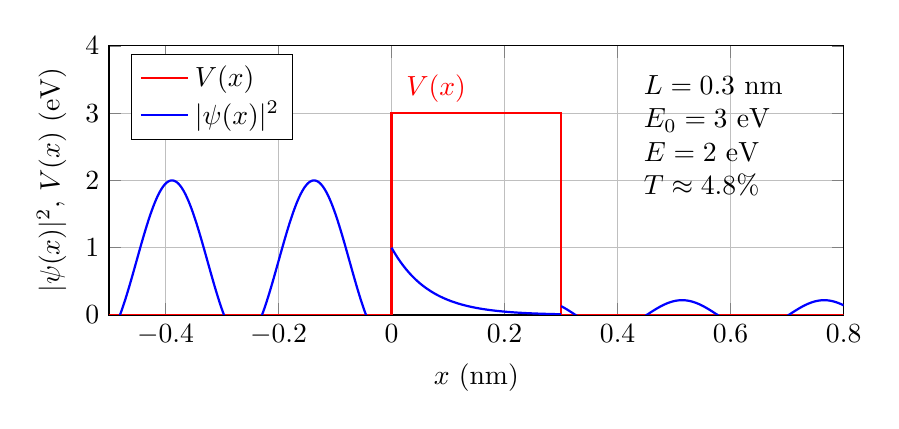
\begin{tikzpicture}
            \begin{axis}
                [
                width=0.9\textwidth,
                height=5cm,
                xlabel=$x$ (nm),
                ylabel={$|\psi(x)|^2$, $V(x)$ (eV)},
                xmin=-0.5, xmax=0.8,
                ymin=0, ymax=4,
                grid=major,
                legend style={cells={anchor=west},legend pos=north west}
                ]

% Potenzialwand zeichnen
                \addplot[red,thick,const plot] coordinates {
                    (-0.5,0)
                    (0,0)
                    (0,3)
                    (0.3,3)
                    (0.3,0)
                    (0.8,0)
                } node[pos=0.5,above left] {$V(x)$};

% Wellenfunktion (qualitativer Verlauf)
                \addplot[blue,thick,samples=200,domain=-0.5:0] {
                    1.2*sin(deg(25*x + 5)) + 0.8 % Bereich I: Links der Wand
                };
                \addplot[blue,thick,samples=200,domain=0:0.3] {
                    1.0*exp(-15*x) % Bereich II: In der Wand (exponentieller Abfall)
                };
                \addplot[blue,thick,samples=200,domain=0.3:0.8] {
                    0.22*sin(deg(25*x - 5)) % Bereich III: Rechts der Wand
                };

% Theoretische Parameter
                \node[anchor=south west] at (0.4,1.5) {
                    \begin{tabular}{l}
                        $L = 0.3$ nm \\
                        $E_0 = 3$ eV \\
                        $E = 2$ eV   \\
                        $T \approx 4.8\%$
                    \end{tabular}
                };

                \legend{$V(x)$, $|\psi(x)|^2$}
            \end{axis}
        \end{tikzpicture}

        \begin{itemize}
            \item Links: Einlaufende + reflektierte Welle ($|A|^2 + |B|^2 \approx 95.2\%$)
            \item Wand: Exponentieller Abfall ($\psi \sim e^{-\kappa x}$)
            \item Rechts: Transmittierte Welle ($|F|^2 \approx 4.8\%$)
        \end{itemize}
    \end{frame}

    \begin{frame}{Zusammenfassung Tunnelformel}
        \begin{itemize}
            \item Exakte Formel enthält hyperbolische Funktionen
            \item Praxisrelevant: Exponentielle Näherung für dicke Barrieren
%            \item Wichtige Parameter:
%            \begin{itemize}
%                \item Barrierenbreite \( L \) (in Metern)
%                \item Höhe der Potenzialbarriere \( E_0 \) (in Joule oder eV)
%                \item Masse des Teilchens \( m \) (in Kilogramm)
%            \end{itemize}
            \item Teilchen kann klassisch unüberwindbare Barrieren durchtunneln
%            \item Experimenteller Nachweis: Strom im Rastertunnelmikroskop fällt exponentiell mit dem Abstand
        \end{itemize}
    \end{frame}

%    \begin{frame}{Physikalische Interpretation}
%        \begin{itemize}
%            \item Teilchen kann klassisch unüberwindbare Barrieren durchtunneln
%            \item Transmissionswahrscheinlichkeit hängt exponentiell ab von:
%            \begin{itemize}
%                \item Barrierenhöhe $(E_0 - E)$
%                \item Barrierenbreite $L$
%            \end{itemize}
%            \item Anwendungen: Rastertunnelmikroskop, Alphazerfall
%        \end{itemize}
%    \end{frame}


%    \begin{frame}{Was ist der Tunneleffekt?}
%        \begin{itemize}
%            \item Elektronen haben eine endliche Wahrscheinlichkeit, durch eine Barriere zu tunneln.
%            \item Besonders relevant bei sehr dünnen Schichten in Mikrochips (unter 1 nm).
%            \item Problematisch bei Gate-Oxiden in Transistoren.
%        \end{itemize}
%    \end{frame}

    \begin{frame}{Beispiel: Siliziumdioxid-Schicht in einem Transistor}
        \textbf{Gegeben:}
        \begin{itemize}
            \item Elektronenenergie: $E = 1.5$ eV
            \item Barrierenhöhe: $E_0 = 3$ eV
            \item Schichtdicke: $L = 0.3$ nm
        \end{itemize}

        \textbf{Korrekte Berechnung:}
        \begin{align*}
            \kappa &= \sqrt{\frac{2m(E_0 - E)}{\hbar^2}} \\
            &= \sqrt{\frac{2 \cdot 9.109 \times 10^{-31} \cdot 2.403 \times 10^{-19}}{(1.055 \times 10^{-34})^2}} \\
            &\approx 6.27 \times 10^9 \, \text{m}^{-1}
        \end{align*}

        \begin{align*}
            T &= e^{-2 \kappa L} = e^{-2 \cdot 6.27 \times 10^9 \cdot 0.3 \times 10^{-9}} \\
            &= e^{-3.76} \approx 0.0235 \, (2.35\%)
        \end{align*}

        \textbf{Ergebnis:} Etwa 2.35\% der Elektronen tunneln durch die Schicht.
    \end{frame}

    \begin{frame}{Auswirkungen auf Mikrochips}
        \begin{itemize}
            \item Leckströme steigen – höhere Verlustleistung
            \item Erwärmung der Chips
            \item Reduzierte Zuverlässigkeit von Transistoren
        \end{itemize}

        \centering
        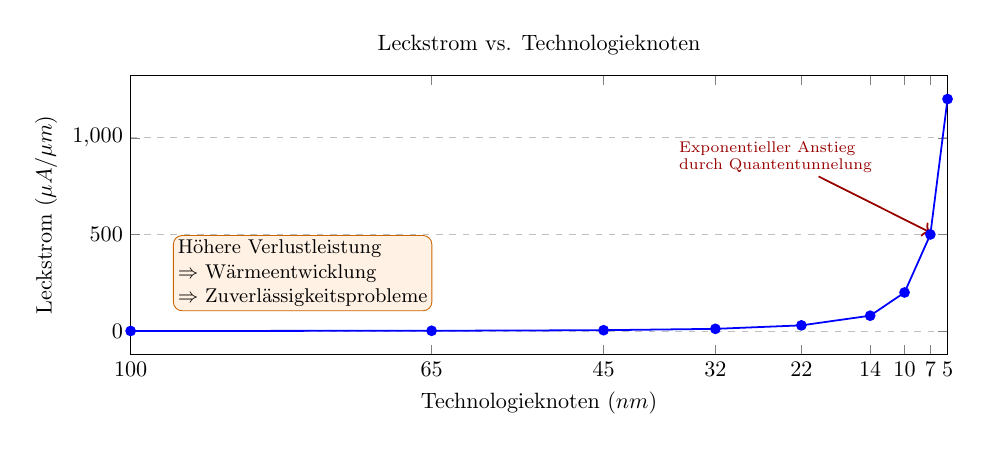
\begin{tikzpicture}[scale=0.8]
            \begin{axis}
                [
                title={Leckstrom vs. Technologieknoten},
                xlabel={Technologieknoten ($nm$)},
                ylabel={Leckstrom ($\mu A/\mu m$)},
                x dir=reverse,
                xtick={100, 65, 45, 32, 22, 14, 10, 7, 5},
                xmin=5, xmax=100,
                ymajorgrids=true,
                grid style=dashed,
                legend pos=north west,
                width=1.2\textwidth,
                height=6cm
                ]
                \addplot[blue, thick, mark=*] coordinates {
                    (100, 1)
                    (65,  2)
                    (45,  5)
                    (32, 12)
                    (22, 30)
                    (14, 80)
                    (10, 200)
                    (7,  500)
                    (5,  1200)
                };

                \node[red!60!black, align=left, font=\scriptsize] at (axis cs:25,900)
                    {Exponentieller Anstieg\\durch Quantentunnelung};
                \draw[->, red!60!black, thick] (axis cs:20,800) -- (axis cs:7,510);

                \node[draw=orange!80!black, fill=orange!10, rounded corners,
                    inner sep=2pt, align=left, font=\small] at (axis cs:80,300)
                    {Höhere Verlustleistung\\$\Rightarrow$ Wärmeentwicklung\\$\Rightarrow$ Zuverlässigkeitsprobleme};
            \end{axis}
        \end{tikzpicture}
    \end{frame}

%    \begin{frame}{Lösung: High-K Materialien}
%        \begin{itemize}
%            \item Siliziumdioxid ($SiO_2$) wird durch High-K-Materialien ersetzt.
%            \item Beispiel: Hafniumdioxid ($HfO_2$) – höhere Barrierenhöhe reduziert das Tunneln.
%            \item Ermöglicht kleinere und effizientere Transistoren.
%        \end{itemize}
%    \end{frame}




    \begin{frame}{Zusammenfassung}
        \begin{enumerate}
            \item Schrödinger-Gleichung in jedem Bereich aufstellen
            \item Allgemeine Lösungen finden
            \item Randbedingungen anwenden
            \item Gleichungssystem lösen
            \item Transmissionswahrscheinlichkeit berechnen
        \end{enumerate}

        Quantenphänomene wie Tunneln zeigen fundamentale Unterschiede zur klassischen Physik!
    \end{frame}

%    change color from blue to green
%    \setbeamercolor{frametitle}{bg=green}
    % Folie 1: Motivation Zeitabhängigkeit
\begin{frame}{Von stationär zu dynamisch}
    \textbf{Limit der zeitunabhängigen SG:}
    \begin{itemize}
        \item Beschreibt nur \alert{stationäre Zustände} ($|\psi|^2$ zeitkonstant)
        \item Beispiel: Elektron im Atom (Grundzustand)
    \end{itemize}

    \textbf{Probleme mit Bewegung:}
    \begin{itemize}
        \item Wie beschreibt man Teilchen, die sich bewegen? (z.B. Elektronenstrahl)
        \item Was passiert bei zeitabhängigen Potenzialen $V(x,t)$?
    \end{itemize}

    \centering
    \alert{$\Rightarrow$ Brauch eine Gleichung für $\psi(x,t)$!}
\end{frame}

% Folie 2: Herleitung der TDSE
\begin{frame}{Herleitung der zeitabhängigen SG}
    \textbf{Ansatz:} Energie-Operator $\hat{E} = i\hbar\frac{\partial}{\partial t}$\\
    Analog zu $\hat{p} = -i\hbar\frac{\partial}{\partial x}$

    \textbf{Energiegleichung:}
    \[
        \underbrace{\hat{H}}_{\text{Hamiltonoperator}} \psi = \underbrace{\hat{E}}_{\text{Energieoperator}} \psi
    \]

    \textbf{Einsetzen der Operatoren:}
    \[
        -\frac{\hbar^2}{2m}\frac{\partial^2 \psi}{\partial x^2} + V(x)\psi = i\hbar\frac{\partial \psi}{\partial t}
    \]

    \textbf{Allgemeine Form:}
    \[
        \boxed{\hat{H}\psi(x,t) = i\hbar\frac{\partial}{\partial t}\psi(x,t)}
    \]
\end{frame}

% Folie 3: Vergleich Zeitabhängig vs. Unabhängig
\begin{frame}{Vergleich der Gleichungen}
    \begin{columns}
        \column{0.5\textwidth}
        \textbf{Zeitunabhängig:}
        \[
            \hat{H}\psi = E\psi
        \]
        \begin{itemize}
            \item Eigenwertgleichung
            \item Lösungen: $\psi_n(x)e^{-iE_n t/\hbar}$
            \item Stationäre Zustände
        \end{itemize}

        \column{0.5\textwidth}
        \textbf{Zeitabhängig:}
        \[
            \hat{H}\psi = i\hbar\dot{\psi}
        \]
        \begin{itemize}
            \item Differentialgleichung 1. Ordnung in $t$
            \item Beschreibt Zeitentwicklung
            \item Allgemeine Lösung: Überlagerung von $\psi_n$
        \end{itemize}
    \end{columns}
\end{frame}

% Folie 4: Lösungsansatz (Separation)
\begin{frame}{Lösungsmethode: Separation der Variablen}
    \textbf{Ansatz:} $\psi(x,t) = \phi(x)T(t)$\\
    Einsetzen in TDSE:
    \[
        \frac{\hat{H}\phi(x)}{\phi(x)} = \frac{i\hbar \dot{T}(t)}{T(t)} = E
    \]

    \textbf{Zwei Gleichungen:}
    \begin{enumerate}
        \item Zeitunabhängige SG: $\hat{H}\phi = E\phi$
        \item Zeitentwicklung: $T(t) = e^{-iEt/\hbar}$
    \end{enumerate}

    \textbf{Vollständige Lösung:}
    \[
        \psi(x,t) = \phi(x)e^{-iEt/\hbar}
    \]
    \begin{itemize}
        \item Phasenfaktor $e^{-iEt/\hbar}$ ändert $|\psi|^2$ nicht
    \end{itemize}
\end{frame}

% Folie 5: Wellenpakete (Vorbereitung Doppelspalt)
\begin{frame}{Wellenpaket-Animation (1D-Zeitentwicklung)}
    \centering
    \begin{animateinline}[
        controls={play, step, stop},
        loop,
        poster=first,
        width=0.8\textwidth
    ]{10} % 10 Frames pro Sekunde
        \multiframe{20}{rt=0.0+0.25} % 20 Frames von t=0 bis t=5
        {
            \begin{tikzpicture}
                \begin{axis}[
                    width=0.8\textwidth,
                    height=6cm,
                    xlabel=$x$,
%                        ylabel=$|\psi(x,t)|^2$,
                    ylabel=$|\psi (x\,t)|^2$,
                    xmin=-3, xmax=3,
                    ymin=0, ymax=1.2,
                    grid=major
                ]
                    % Hüllkurve
                    \addplot[red!50, thick, domain=-3:3, samples=50] {
                        exp(-(x - 0.5*\rt)^2)
                    };

                    % Wellenpaket mit Oszillationen
                    \addplot[blue, thick, domain=-3:3, samples=100] {
                        exp(-(x - 0.5*\rt)^2) * (1 + 0.3*cos(deg(5*x - 2*\rt)))
                    };

%                         Zeitmarker
                    \node[draw] at (axis cs:2,1) {$t = \pgfmathprintnumber{\rt}$};
                \end{axis}
            \end{tikzpicture}
        }
    \end{animateinline}

%        \begin{itemize}
%            \item Klicken Sie auf "Play" um die Zeitentwicklung zu starten
%            \item Geschwindigkeit mit "+/-" anpassbar
%            \item Deutlich sichtbar: Bewegung + Dispersion + Interferenz
%        \end{itemize}
\end{frame}

\begin{frame}{Wellenpaket-Animation (2D-Zeitentwicklung)}
    \centering
    \begin{animateinline}[
        controls={play, step, stop},
        loop,
        poster=first,
        width=0.8\textwidth
    ]{10} % 10 Frames pro Sekunde
        \multiframe{20}{rt=0.0+0.25} % 20 Frames von t=0 bis t=5
        {
            \centering
            \begin{tikzpicture}
                \begin{axis}
                    [
                    width=0.8\textwidth,
                    height=6cm,
                    colormap/viridis,
                    view = {45}{30},
                    xlabel = $x$,
                    ylabel = $y$,
                    axis line style={draw=none},
                    zlabel = {Wahrscheinlichkeitsdichte $|\psi(x,y)|^2$},
                    label style = {sloped},
                    grid = major,
                    grid style = {dashed, gray!30},
                    tick label style = {font=\scriptsize},
                    title = {Moduliertes Gaußsches Wellenpaket},
                    title style = {font=\small},
                    colorbar,
                    colorbar style={
                        title=Intensität,
                        yticklabel style={/pgf/number format/.cd,fixed,precision=2}
                    }
                    ]

                    % Hüllkurve
                    \addplot3[
                    surf,
                    shader = interp,
                    samples = 20,
                    domain = -3:3,
                    y domain = -3:3,
%                point meta=abs,
                    ] {
%                    exp(-(x^2 + y^2))       % Gaußscher Kern
%                    * (1 + 0.4*cos(6*x))    % Wellenmodulation
%                    * (1 + 0.4*cos(6*y))    % 2D-Interferenzmuster
%                    exp(-(x^2 + y^2))* (1 + 0.4*cos(6*x))* (1 + 0.4*cos(6*y))
%                        (1 + 0.4*cos(6* deg(x)))* (1 + 0.4*cos(6*deg(y))) * exp(-(x^2 + y^2))
                        exp(-((x - 0.5*\rt)^2 + (y)^2))
                    };


%                    (1 + 0.4*cos(6* deg(x)))* (1 + 0.4*cos(6*deg(y))) * exp(-(x^2 + y^2))
%                    % Hüllkurve
%                    \addplot[red!50, thick, domain=-3:3, samples=50] {
%                        exp(-(x - 0.5*\rt)^2)
%                    };

%                    % Wellenpaket mit Oszillationen
%                    \addplot[blue, thick, domain=-3:3, samples=100] {
%                        exp(-((x - 0.5*\rt)^2)) * (1 + 0.3*cos(deg(5*x - 2*\rt)))
%                    };

%                    \node[white,font=\tiny] at (axis cs:-2.5,-2.5,0.7)
%                        {$\psi(x,y) = e^{-(x^2+y^2)}(1 + 0.4\cos 6x)(1 + 0.4\cos 6y)$};
                \end{axis}
%            \end{tikzpicture}
%            \begin{tikzpicture}
%                \begin{axis}[
%                    width=0.8\textwidth,
%                    height=6cm,
%                    xlabel=$x$,
%%                        ylabel=$|\psi(x,t)|^2$,
%                    ylabel=$|\psi (x\,t)|^2$,
%                    xmin=-3, xmax=3,
%                    ymin=0, ymax=1.2,
%                    grid=major
%                ]
%
%%                    (1 + 0.4*cos(6* deg(x)))* (1 + 0.4*cos(6*deg(y))) * exp(-(x^2 + y^2))
%                    % Hüllkurve
%                    \addplot[red!50, thick, domain=-3:3, samples=50] {
%                        exp(-(x - 0.5*\rt)^2)
%                    };
%
%                    % Wellenpaket mit Oszillationen
%                    \addplot[blue, thick, domain=-3:3, samples=100] {
%                        exp(-((x - 0.5*\rt)^2)) * (1 + 0.3*cos(deg(5*x - 2*\rt)))
%                    };
%
%%                         Zeitmarker
%                    \node[draw] at (axis cs:2,1) {$t = \pgfmathprintnumber{\rt}$};
%                \end{axis}
            \end{tikzpicture}
        }
    \end{animateinline}

%        \begin{itemize}
%            \item Klicken Sie auf "Play" um die Zeitentwicklung zu starten
%            \item Geschwindigkeit mit "+/-" anpassbar
%            \item Deutlich sichtbar: Bewegung + Dispersion + Interferenz
%        \end{itemize}
\end{frame}
% Folie 6: Doppelspalt-Experiment vorbereiten
\begin{frame}{Der Weg zum Doppelspalt}
    \textbf{Modellierung im 2D:}
    \[
        i\hbar\frac{\partial \psi}{\partial t} = \left(-\frac{\hbar^2}{2m}(\frac{\partial^2}{\partial x^2} + \frac{\partial^2}{\partial y^2}) + V(x,y)\right)\psi
    \]

    \textbf{Potenzial beim Doppelspalt:}
    \[
        V(x,y) = \begin{cases}
                     \infty & \text{(Wand)} \\
                     0 & \text{(Spalte)}
        \end{cases}
    \]

    \textbf{Lösungsstrategie:}
    \begin{enumerate}
        \item Anfangsbedingung: Wellenpaket vor der Wand
        \item Zeitentwicklung berechnen (numerisch)
        \item Interferenzmuster entsteht durch $\psi_1 + \psi_2$
    \end{enumerate}
\end{frame}


\begin{frame}{Doppelspaltexperiment – Live-Animation}
    \centering
%\movie[width=0.8\textwidth,height=0.6\textwidth,poster,showcontrols]{}{../double_slit.gif}

    \animategraphics[loop,controls,width=\linewidth]{10}{./render/frame_}{0000}{0199}


%\begin{itemize}
%    \item Wellenausbreitung durch beide Spalte
%    \item Interferenzmuster entsteht am Detektor
%    \item Typisches Quantenphänomen: Selbstinterferenz
%\end{itemize}
\end{frame}

    % Folie 1: Vom Wasserstoffatom zu Mehrelektronensystemen
\begin{frame}{Grundlagen atomarer Orbitale}
    \textbf{Wasserstoffatom (exakt lösbar):}
    \begin{itemize}
        \item Zeitunabhängige SG: $\left(-\frac{\hbar^2}{2\mu}\nabla^2 - \frac{e^2}{4\pi\epsilon_0 r}\right)\psi = E\psi$
        \item Lösung: $\psi_{nlm}(r,\theta,\phi) = R_{nl}(r)Y_l^m(\theta,\phi)$
        \item Quantenzahlen: $n,l,m$
    \end{itemize}

    \begin{columns}
        \column{0.5\textwidth}
        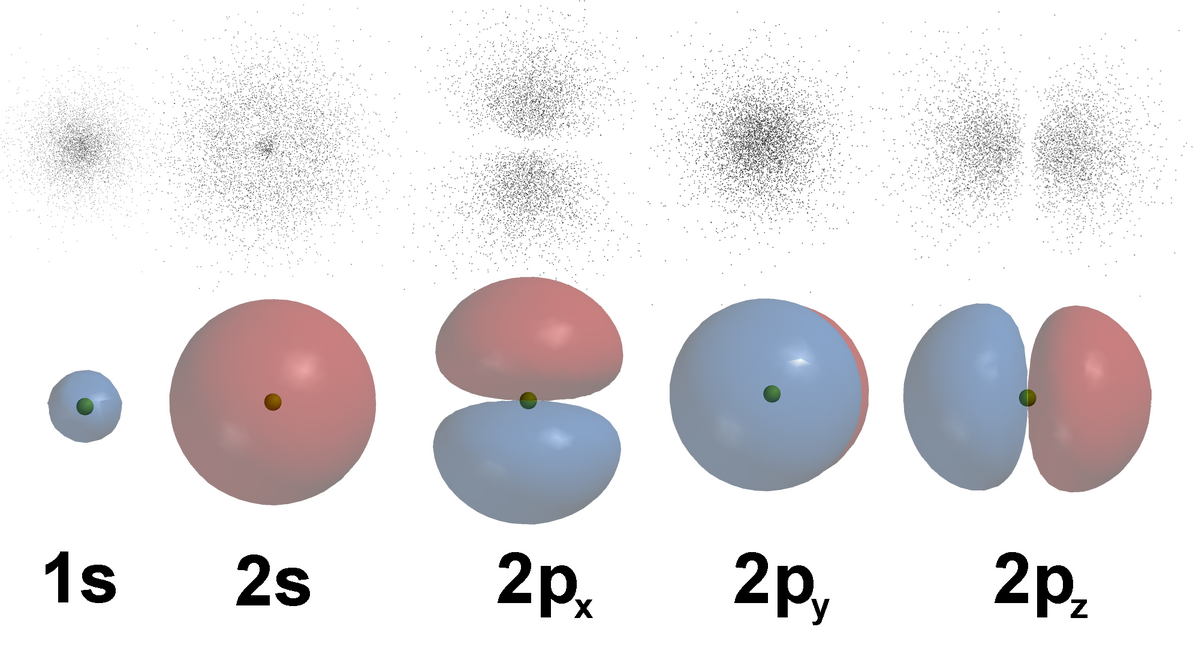
\includegraphics[width=\textwidth]{orbitals.png}

        \column{0.5\textwidth}
        \begin{itemize}
            \item Radialteil $R_{nl}(r)$
            \item Winkelteil $Y_l^m(\theta,\phi)$
        \end{itemize}
    \end{columns}
\end{frame}

% Folie 2: Das Mehrelektronenproblem
\begin{frame}{Die Herausforderung bei Mehrelektronenatomen}
    \textbf{Schrödinger-Gleichung:}
    \[
        \hat{H} = \sum_i \left(-\frac{\hbar^2}{2m}\nabla_i^2 - \frac{Ze^2}{4\pi\epsilon_0 r_i}\right) + \sum_{i<j} \frac{e^2}{4\pi\epsilon_0 r_{ij}}
    \]

    \begin{itemize}
        \item Elektron-Elektron-Wechselwirkung macht Gleichung unlösbar
        \item \alert{Approximationsmethoden} erforderlich:
        \begin{itemize}
            \item Hartree-Fock-Methode
            \item Dichtefunktionaltheorie (DFT)
        \end{itemize}
    \end{itemize}
\end{frame}

% Folie 3: Hartree-Fock-Methode
\begin{frame}{Hartree-Fock-Approximation}
    \textbf{Key Ideas:}
    \begin{itemize}
        \item Jedes Elektron bewegt sich im gemittelten Feld der anderen
        \item Slater-Determinante für Antisymmetrie
    \end{itemize}

    \textbf{Hartree-Fock-Gleichungen:}
    \[
        \hat{F}\phi_i(1) = \epsilon_i\phi_i(1)
    \]
    Fock-Operator:
    \[
        \hat{F} = \hat{h} + \sum_j (\hat{J}_j - \hat{K}_j)
    \]
    \begin{itemize}
        \item $\hat{J}_j$: Coulomb-Operator
        \item $\hat{K}_j$: Austauschoperator
    \end{itemize}
\end{frame}

% Folie 4: Dichtefunktionaltheorie
\begin{frame}{Dichtefunktionaltheorie (DFT)}
    \textbf{Hohenberg-Kohn-Theorem:}
    \begin{itemize}
        \item Grundzustandsenergie ist Funktional der Elektronendichte
        \item $E[n(\vec{r})] = T[n] + V_{ext}[n] + E_{ee}[n]$
    \end{itemize}

    \textbf{Kohn-Sham-Gleichungen:}
    \[
        \left(-\frac{\hbar^2}{2m}\nabla^2 + v_{eff}(\vec{r})\right)\psi_i = \epsilon_i\psi_i
    \]
    Effektives Potenzial:
    \[
        v_{eff} = v_{ext} + \int \frac{n(\vec{r}')}{|\vec{r}-\vec{r}'|}d\vec{r}' + v_{xc}[n]
    \]
\end{frame}

% Folie 5: Numerische Berechnung
\begin{frame}{Vom Konzept zur Berechnung}
    \textbf{Praktische Umsetzung:}
    \begin{itemize}
        \item Basis-Sätze (Gauß-Funktionen, planewaves)
        \item Selbstkonsistente Feld-Iteration
        \item Software-Pakete: Gaussian, VASP, Quantum ESPRESSO
    \end{itemize}

%    \begin{block}{Berechnungsschritte}
%        \begin{enumerate}
%            \item Start mit Trial-Dichte
%            \item Löse Kohn-Sham-Gleichungen
%            \item Aktualisiere Dichte
%            \item Wiederhole bis Konvergenz
%        \end{enumerate}
%    \end{block}
\end{frame}

% Folie 6: Zusammenfassung
%\begin{frame}{Zusammenfassung Orbitalberechnung}
%    \begin{itemize}
%        \item \textbf{Exakte Lösung} nur für Wasserstoff möglich
%        \item \textbf{Hartree-Fock}: Berücksichtigt Austauchwechselwirkung
%        \item \textbf{DFT}: Arbeitet mit Elektronendichte statt Wellenfunktion
%        \item \textbf{Numerische Methoden}: Basis-Sätze + iterative Lösungen
%    \end{itemize}
%
%    \centering
%%    \includegraphics[width=0.5\textwidth]{dft_flowchart.png}
%
%    \begin{tikzpicture}[
%        node distance=1.5cm,
%        startstop/.style={rectangle, rounded corners, minimum width=3cm, minimum height=1cm, text centered, draw=black, fill=red!30},
%        process/.style={rectangle, minimum width=3cm, minimum height=1cm, text centered, draw=black, fill=blue!30},
%        decision/.style={diamond, aspect=1.5, minimum width=2cm, minimum height=1cm, text centered, draw=black, fill=green!30},
%        arrow/.style={-Stealth[scale=1.2]},
%        annotation/.style={font=\scriptsize, text width=2cm}
%    ]
%
%% Nodes
%        \node (start) [startstop] {Start};
%        \node (init) [process, below=of start] {Initial guess\\$n^{(0)}(\vec{r})$};
%        \node (potential) [process, below=of init] {Berechne\\$v_{eff}[n^{(i)}]$};
%        \node (solve) [process, below=of potential] {Löse Kohn-Sham\\Gleichungen};
%        \node (update) [process, below=of solve] {Aktualisiere Dichte\\$n^{(i+1)}(\vec{r})$};
%        \node (decide) [decision, below=of update] {Konvergenz?\\$|n^{(i+1)}-n^{(i)}| < \epsilon$};
%        \node (end) [startstop, below=of decide] {Ausgabe:\\Energie, Orbitale};
%
%% Annotations
%        \node [annotation, right=1cm of potential] {
%            \begin{itemize}
%                \item[] LDA/GGA
%                \item[] $v_{xc}[n]$
%            \end{itemize}
%        };
%
%        \node [annotation, left=1cm of solve] {
%            \begin{itemize}
%                \item[] Gauß-Basis
%                \item[] Plane waves
%            \end{itemize}
%        };
%
%% Arrows
%        \draw [arrow] (start) -- (init);
%        \draw [arrow] (init) -- (potential);
%        \draw [arrow] (potential) -- (solve);
%        \draw [arrow] (solve) -- (update);
%        \draw [arrow] (update) -- (decide);
%        \draw [arrow] (decide) -- node[right] {Ja} (end);
%        \draw [arrow] (decide.east) -- ++(2,0) |- node[near start, above] {Nein} (potential.east);
%
%% Loop label
%        \draw [stealth-stealth, dotted] (potential.east) ++(1.5,0) -- ++(0,3.5) node[midway, right, annotation] {
%            Selbstkonsistente\\Iteration
%        };
%
%    \end{tikzpicture}
%
%\end{frame}

    \begin{frame}
        \centering
        \Huge
        \textcolor{black}{Vielen Dank für Ihre Aufmerksamkeit!}
    \end{frame}
\end{document}